%!TEX TS-program = xelatex
\documentclass[10pt]{article}
\usepackage[a4paper,margin=0mm]{geometry}
\usepackage{fontspec}
\usepackage{tikz}
\usepackage{amsmath}
\usepackage{amssymb}
\usepackage{graphicx}
\graphicspath{{text/application/assets/}{assets/}}
\usepackage{xcolor}
\usepackage[protrusion=true,expansion=false]{microtype}
\usepackage{ragged2e}
\usepackage{qrcode}
\usepackage{eso-pic}
\usepackage{setspace}
\usepackage{calc}
\usepackage{array}
\usepackage{hyperref}
\hypersetup{hidelinks}

\setmainfont{lmroman10-regular.otf}[
  Path=/usr/local/texlive/2024/texmf-dist/fonts/opentype/public/lm/,
  BoldFont=lmroman10-bold.otf,
  ItalicFont=lmroman10-italic.otf,
  BoldItalicFont=lmroman10-bolditalic.otf]
\newfontfamily\metafont{lmroman10-regular.otf}[
  Path=/usr/local/texlive/2024/texmf-dist/fonts/opentype/public/lm/,
  Scale=MatchLowercase]
\newcommand{\displayfont}{\rmfamily\bfseries}
\definecolor{paper}{HTML}{FFFFFF}
\definecolor{ink}{HTML}{000000}
\definecolor{signal}{HTML}{000000}
\pagecolor{paper}\color{ink}
\pagestyle{empty}
\setlength{\parindent}{0pt}

\newcommand{\meta}[2]{%
  \begin{tikzpicture}[remember picture,overlay]
    \draw[signal,line width=.55pt] ([xshift=11mm,yshift=-11mm]current page.north west) rectangle ++(44mm,-17mm);
    \node[anchor=north west,align=left,font=\metafont\fontsize{6.2}{7.2}\selectfont] at ([xshift=13mm,yshift=-13mm]current page.north west) {TAKE OVER\\FOTOGRAFISKA TALLINN\\#1};
    \node[anchor=north east,text=signal,font=\metafont\fontsize{6.2}{7.2}\selectfont] at ([xshift=53mm,yshift=-25mm]current page.north west) {#2};
  \end{tikzpicture}\par}

\newcommand{\folio}[1]{\begin{tikzpicture}[remember picture,overlay]
\node[anchor=south east,text=signal,font=\metafont\fontsize{6}{7}\selectfont] at ([xshift=-10mm,yshift=8mm]current page.south east) {#1 / 18};
\end{tikzpicture}\par}

\newcommand{\statement}[1]{{\RaggedRight\displayfont\color{signal}\fontsize{36}{34}\selectfont\MakeUppercase{#1}\par}}
\newcommand{\bigstatement}[1]{{\RaggedRight\displayfont\color{signal}\fontsize{55}{51}\selectfont\MakeUppercase{#1}\par}}
\newcommand{\smallcapsline}[1]{{\metafont\color{signal}\fontsize{7}{9}\selectfont\MakeUppercase{#1}}}
\newcommand{\sectionnumber}[1]{{\rmfamily\bfseries\color{signal}\fontsize{28}{28}\selectfont #1.}}
\newcommand{\sidelegend}{\begin{tikzpicture}[remember picture,overlay]
  \node[rotate=90,anchor=south west,text=signal,font=\rmfamily\bfseries\fontsize{7}{8}\selectfont]
  at ([xshift=10mm,yshift=12mm]current page.south west)
  {IMAGE / VOICE / PLACE / PRACTICE / RELATION / NEXT};
  \draw[signal,line width=.5pt] ([xshift=11mm,yshift=12mm]current page.south west)--([xshift=11mm,yshift=82mm]current page.south west);
\end{tikzpicture}\par}

\newcommand{\photobox}[2][.72\paperheight]{%
  \begin{tikzpicture}
    \fill[white] (0,0) rectangle (\linewidth-.8pt,#1);
    \draw[signal,line width=.7pt] (0,0) rectangle (\linewidth-.8pt,#1);
    \draw[signal,line width=.35pt] (0,0)--(\linewidth-.8pt,#1) (0,#1)--(\linewidth-.8pt,0);
    \node[fill=paper,inner sep=4mm,align=center,text=signal,font=\metafont\fontsize{8}{10}\selectfont] at (.5\linewidth-.4pt,.5#1) {PHOTOGRAPH PLACEHOLDER\\#2};
  \end{tikzpicture}}

\newcommand{\networkbg}[1]{%
\begin{tikzpicture}[remember picture,overlay]
\foreach \x/\y in {20/25,44/18,72/28,88/46,67/67,38/72,16/58}{\fill[black] ([xshift=\x mm,yshift=\y mm]current page.south west) circle (.8pt);}
\draw[black,line width=.25pt] ([xshift=20mm,yshift=25mm]current page.south west)--([xshift=44mm,yshift=18mm]current page.south west)--([xshift=72mm,yshift=28mm]current page.south west)--([xshift=88mm,yshift=46mm]current page.south west);
\draw[black,line width=.25pt] ([xshift=44mm,yshift=18mm]current page.south west)--([xshift=67mm,yshift=67mm]current page.south west)--([xshift=38mm,yshift=72mm]current page.south west)--([xshift=16mm,yshift=58mm]current page.south west);
\end{tikzpicture}\par}

\begin{document}

% 1 START
\meta{COMMUNITY GALLERY}{START}\folio{01}\sidelegend
\vspace*{55mm}
\begin{center}
  {\rmfamily\itshape\fontsize{12}{15}\selectfont (the process of)}\par
  \vspace{5mm}
  {\rmfamily\bfseries\fontsize{90}{88}\selectfont +\kern-.08em*\kern-.08em/}\par
  \vspace{7mm}
  {\metafont\fontsize{9}{12}\selectfont INTERACTIVE IN PROGRESS}\par
  \vspace{16mm}
  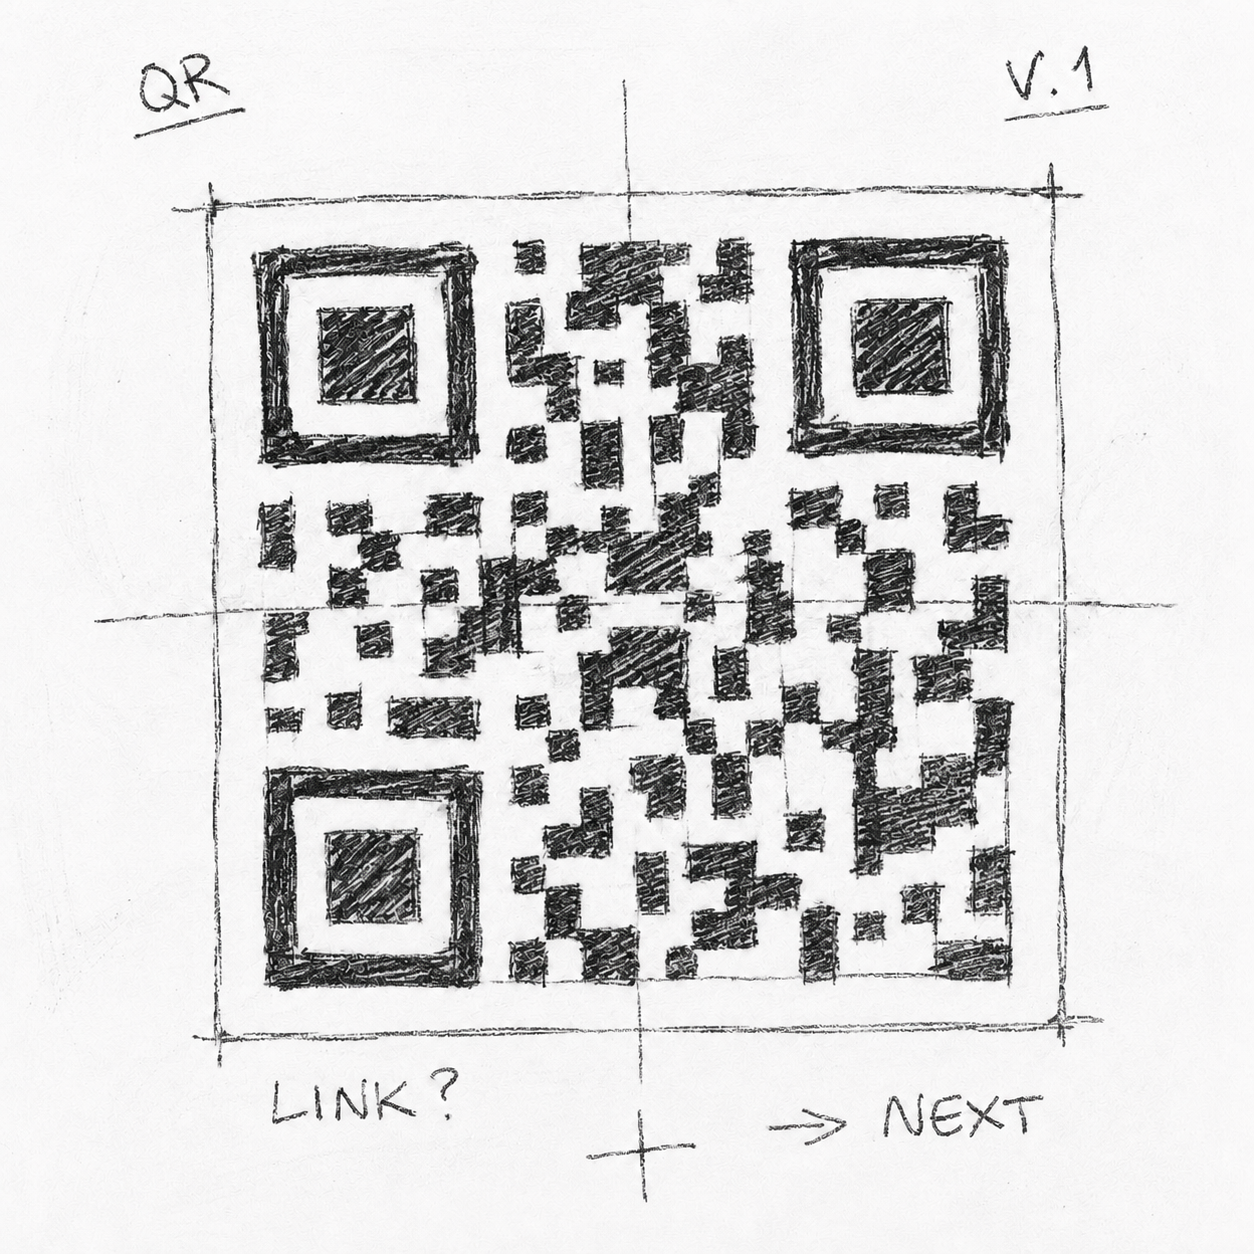
\includegraphics[width=46mm]{qr_sketch_inverted.png}
\end{center}
\vfill
\hspace*{14mm}\smallcapsline{This application is the first event in the process.}\vspace{15mm}
\newpage

% 2 CHIME
\meta{INITIAL CONDITION}{CHIME}\folio{02}\sidelegend
\begin{tikzpicture}[remember picture,overlay]
  \node[anchor=north west,align=left,text width=38mm,font=\fontsize{8.8}{11.2}\selectfont]
  at ([xshift=14mm,yshift=168mm]current page.south west) {%
    \textbf{TAKE OVER is an initial condition looking for consequences.}\\[5mm]
    \textbf{WHAT IS THIS NOT?}\\[3mm]
    Everything asks to be continued.\\
    Enter anywhere.\\
    Change what follows.};
\end{tikzpicture}\par
\vspace*{46mm}\hspace*{62mm}
\begin{minipage}{128mm}
  \bigstatement{TAKE\\OVER.}
  \vspace{8mm}
  {\fontsize{17}{22}\selectfont through the \textbf{WALL}.}\par
  \vspace{18mm}
  {\fontsize{18}{24}\selectfont
    image $\rightarrow$ voice $\rightarrow$ sound\\
    $\rightarrow$ person $\rightarrow$ practice\\
    $\rightarrow$ relation $\rightarrow$ next}
  \par\vspace{18mm}
  {\fontsize{13}{17}\selectfont\itshape an initial condition.}\par
\end{minipage}
\newpage

% 3 ABSTRACT
\meta{APPLICATION}{INITIAL CONDITION}\folio{03}\sidelegend
\vspace*{45mm}\hspace*{62mm}
\begin{minipage}{128mm}
  \sectionnumber{0}\par\vspace{1mm}
  {\displayfont\color{signal}\fontsize{24}{24}\selectfont INITIAL CONDITION.}\par\vspace{8mm}
  {\fontsize{12.5}{16}\selectfont
    A photographic sequence of abandoned churches, damaged architectures, bodies, apertures, and objects whose meaning changes as they carry on, frame to frame.\\[5mm]
    Beside and within the photographic work, encoded portals open another layer: voices, field recordings and other sounds. The image does not explain; the sound does not close it. Each can spark another connection.\\[5mm]
    TAKE OVER begins from what remains. We inherit architectures, images, memories, relationships, sounds, and debris. It asks what can begin inside spaces opened by something else. Community is a process.
  }
\end{minipage}
\newpage

% 4 RATIONALE
\meta{RATIONALE}{ENTRY 00}\folio{04}\sidelegend
\vspace*{51mm}\hspace*{21mm}
\begin{minipage}{168mm}
  \setlength{\parindent}{0pt}
  \justifying
  {\fontsize{18}{23}\selectfont
    \hangindent=13mm\hangafter=1
    \textbf{rationale}\enspace \textit{n.}\enspace
    From what remains: architectures, images, memories, relationships, sounds,
    and debris. TAKE OVER asks what can begin inside spaces opened by something
    else. --- Community is not presented as a stable object but as a process.
    Photography opens to voice; voice opens to sound. Sound opens to another
    person; another person brings another practice. The work grows through these
    relations.\par}
  \vspace{13mm}
  {\fontsize{14}{19}\selectfont
    \textbf{Deriv.}\enspace
    \textit{image-to-voice; voice-to-sound; sound-to-person; person-to-practice;
    practice-to-relation; relation-to-next.}\par}
  \vspace{38mm}
  {\fontsize{12}{16}\selectfont
    An initial condition looking for consequences. Everything asks to be
    continued. Enter anywhere. Change what follows.}
\end{minipage}
\newpage

% 5 SYSTEM
\meta{SYSTEM}{PERTURBATION}\folio{05}\sidelegend
\vspace*{57mm}
\begin{center}
  {\fontsize{38}{45}\selectfont
    \[
      7+5+\cdots=12
    \]}
  \vspace{16mm}
  {\fontsize{13}{17}\selectfont\itshape initial allocation}\par
  \vspace{30mm}
  {\fontsize{38}{45}\selectfont
    \[
      12+\square+\square+\square=15
    \]}
  \vspace{16mm}
  {\fontsize{13}{17}\selectfont\itshape positions reserved for what has not surfaced yet}\par
\end{center}
\newpage

% 5 EXHIBITION
\meta{EXHIBITION}{SYSTEM OF RELATIONS}\folio{06}\sidelegend
\vspace*{43mm}\hspace*{62mm}
\begin{minipage}{128mm}
  {\RaggedRight\displayfont\fontsize{27}{28}\selectfont THE WALL IS THE\\INITIAL CONDITION.}\par
  \vspace{9mm}
  {\fontsize{11.5}{15}\selectfont
    The exhibition combines photographic works by the initial contributors with small QR portals connecting selected works to voices, sound, and the evolving digital surface. It does not attempt to fill every available position. Some positions remain unallocated: scarce exhibition space is reserved for contributions that have not surfaced yet.}
\end{minipage}\par
\vspace{12mm}
\hspace*{14mm}\begin{minipage}{182mm}
  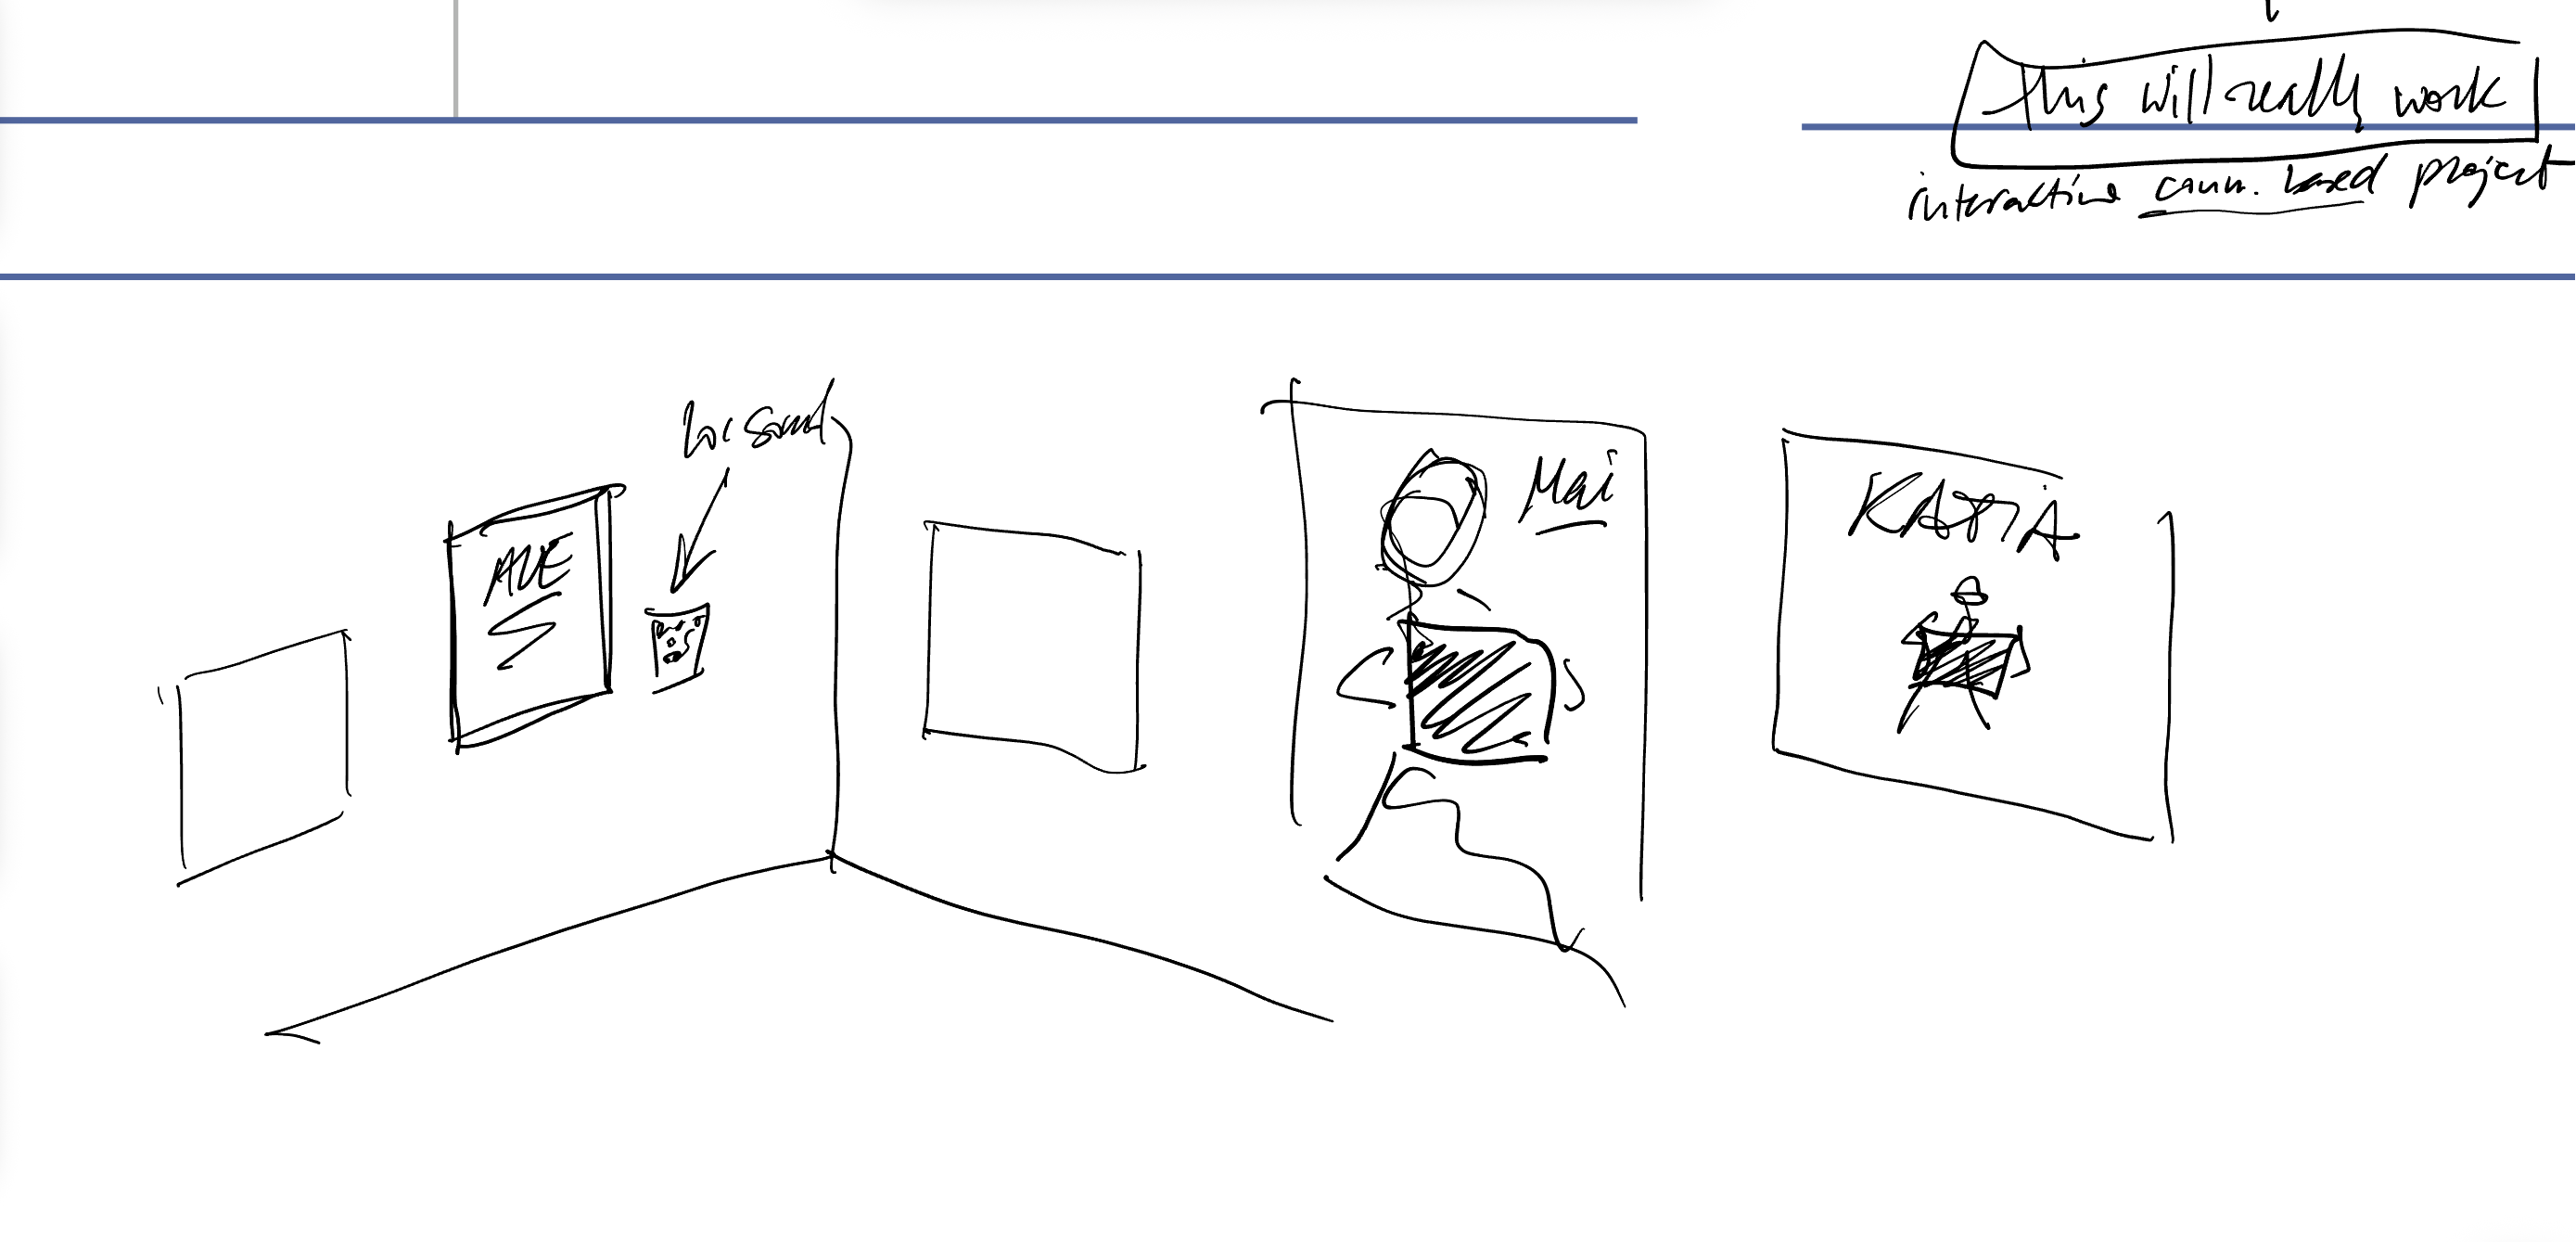
\includegraphics[width=182mm,trim=55 35 75 245,clip]{assets/exhibition.png}\par
  \vspace{3mm}
  \smallcapsline{Fig. 1 / A system of relations, not a hanging plan.}
\end{minipage}
\newpage

% 5 PHOTO
\meta{PHOTOGRAPH}{NODE 01}\folio{07}\sidelegend
\vspace*{36mm}\hspace*{14mm}
\begin{minipage}{179mm}
  \photobox[205mm]{KUMIORI / ABANDONED CHURCH / SELECTED SEQUENCE}
  \vspace{4mm}
  \smallcapsline{Architectures / bodies / apertures / objects / frame to frame.}
\end{minipage}
\newpage

% 6 VOICE
\meta{VOICE}{NODE 01 / AUDIO}\folio{08}\sidelegend
\vspace*{47mm}\hspace*{62mm}
\begin{minipage}{128mm}
  \statement{THE IMAGE\\DOES NOT\\EXPLAIN.}\par
  \vspace{24mm}
  \begin{minipage}{78mm}
    {\fontsize{13}{17}\selectfont\itshape
    ``Mai-Brit Tänava enters in the frame and through voice. Her recorded contribution opens another perspective from inside it.''}
  \end{minipage}
  \hfill
  \begin{minipage}{35mm}\centering
    \qrcode[height=30mm]{https://example.org/takeover/mai}\par\vspace{3mm}
    \smallcapsline{LISTEN}
  \end{minipage}
\end{minipage}
\newpage

% 7 MULTIPLEX
\meta{SYSTEM}{MULTIPLEX}\folio{09}\sidelegend
\vspace*{45mm}\hspace*{62mm}
\begin{minipage}{128mm}
  \sectionnumber{1}\par\vspace{1mm}
  {\RaggedRight\displayfont\color{signal}\fontsize{23}{24}\selectfont WHAT GROWS BETWEEN THEM\\IS THE WORK.}\par
  \vspace{18mm}
  {\color{signal}\fontsize{18}{26}\selectfont
    \[
      \mathcal W=\{\mathrm{image},\mathrm{voice},\mathrm{sound},\mathrm{body},\ldots\}-\mathcal R
    \]}
  \vspace{22mm}
  {\fontsize{11.5}{15}\selectfont
  TAKE OVER begins as an individual application that is already becoming something else. Andrés A. León Baldelli / KUMIORI, Ave Palm, Mai-Brit Tänava, and Kenn-Eerik Kannike remain attributable authors. Their contributions are not merged into anonymous collective authorship. Here, $\mathcal R$ is not fixed in advance: it is the evolving set of relations between contributors, works, places, and encounters.}
\end{minipage}
\newpage

% 8 EMPTY
\meta{VACANCY}{OPEN NODE}\folio{10}\sidelegend
\vspace*{54mm}\hspace*{14mm}
\begin{minipage}{179mm}
  \statement{UNALLOCATED\\IS NOT EMPTY.}\par
  \vspace{92mm}
  {\fontsize{18}{23}\selectfont\itshape Not because material is missing. Because somebody is.}\par
  \vspace{12mm}
  {\fontsize{34}{42}\selectfont\[\text{WHO ENTERS NEXT?}\]}
\end{minipage}
\newpage

% 9 PHOTO 2
\meta{PHOTOGRAPH}{NODE 02}\folio{11}\sidelegend
\vspace*{36mm}\hspace*{14mm}
\begin{minipage}{180mm}
  \photobox[205mm]{AVE PALM / PROVISIONAL SELECTION}
  \vspace{4mm}
  \smallcapsline{Abandoned architectures / bodies / movement / cyanotype.}
\end{minipage}
\newpage

% 10 SOUND
\meta{SOUND}{NODE 03}\folio{12}\sidelegend
\begin{tikzpicture}[remember picture,overlay]
  \node[anchor=north west,align=left,text width=38mm,
        font=\fontsize{8.5}{11}\selectfont]
    at ([xshift=14mm,yshift=-92mm]current page.north west)
    {\textbf{ARVO P\"ART}\\[-.5mm]\textit{Ludus}\\[1.5mm]\textit{``game'' in Latin}};
\end{tikzpicture}
\vspace*{47mm}\hspace*{62mm}
\begin{minipage}{128mm}
  \bigstatement{LISTEN.}\par
  \vspace{18mm}
  {\fontsize{14}{19}\selectfont
    Sound is location and grounding. Some QR portals carry recordings made at or in relation to the photographed sites; others carry voices or composed material. Kenn-Eerik Kannike develops the sonic trajectory through recordings, listening, and live electronic concert.}
  \vspace{24mm}
  \begin{center}
    \begin{tikzpicture}[x=1cm,y=1cm]
      \node[anchor=south west,inner sep=0] at (0,0)
        {
\includegraphics[width=12cm,height=1.8cm]{../../fig/listen_waveform_clean.png}};
      \node[anchor=north,text=signal,font=\metafont\fontsize{7}{9}\selectfont] at (2.05,-.35) {CHIRP};
      \node[anchor=north,text=signal,font=\metafont\fontsize{7}{9}\selectfont] at (4.85,-.35) {SILENCE};
      \node[anchor=north east,text=signal,font=\metafont\fontsize{7}{9}\selectfont] at (12,-.35) {SMOOTH CRESCENDO};
    \end{tikzpicture}
  \end{center}
\end{minipage}
\newpage

% 11 TRAJECTORY
\meta{TRAJECTORY}{TIMELINE}\folio{13}\sidelegend
\vspace*{45mm}\hspace*{62mm}
\begin{minipage}{128mm}
  \sectionnumber{2}\par\vspace{1mm}
  {\RaggedRight\displayfont\color{signal}\fontsize{23}{24}\selectfont THE OPENING CHANGES\\THE EXHIBITION.}\par
  \vspace{24mm}
  \begin{tikzpicture}[x=1mm,y=1mm]
    \draw[signal,line width=.8pt] (0,0)--(121,0);
    \foreach \x/\lab in {1/APPLY,28/HUMAN,59/OPENING,91/NIGHT,121/?}{\fill[signal] (\x,0) circle (1.7pt);\node[anchor=north,text=signal,font=\metafont\fontsize{6.5}{8}\selectfont] at (\x,-4) {\lab};}
    \draw[signal,dashed,line width=.5pt] (59,-18)--(59,38);
    \node[anchor=south west,align=left,text width=50mm,font=\fontsize{11}{14}\selectfont] at (61,10) {photography + voice +\\situated sound + movement};
  \end{tikzpicture}
  \vspace{34mm}
  {\fontsize{12}{16}\selectfont Concert, live sound, performance, food, and night are possible consequences, not requirements. Each practice enters as someone brings it. Something happens. There is an interval. What follows is changed by it.}
\end{minipage}
\newpage

% 12 NEEDS
\meta{NECESSITIES}{CURRENT STATE}\folio{14}\sidelegend
\vspace*{45mm}\hspace*{62mm}
\begin{minipage}{128mm}
  \statement{CURRENT\\STATE.}\par
  \vspace{18mm}
  \renewcommand{\arraystretch}{1.7}
  \setlength{\tabcolsep}{1.5mm}
  \begin{tabular}{>{\metafont\fontsize{6.5}{8}\selectfont}p{23mm} p{69mm} >{\raggedleft\arraybackslash}p{25mm}}
    ELEMENT     & CONDITION                         & STATUS         \\ \hline
    PHOTOGRAPHS & initial sequence                  & SELECTED       \\
    AVE         & photographic contribution         & IN PROGRESS    \\
    VOICE       & initial contribution              & AGREED         \\
    SOUND       & field recordings / collaboration  & AGREED         \\
    WEB SURFACE & operational prototype             & IN DEVELOPMENT \\
    QR / PORTAL & concept / visual language         & ESTABLISHED    \\
    UNALLOCATED & photographic and exhibition space & OPEN           \\
  \end{tabular}
\end{minipage}
\newpage

% 13 GRAPH
\meta{PROPAGATION}{STATE $G_n$}\folio{15}\sidelegend
\networkbg{22}
\vspace*{45mm}\hspace*{62mm}
\begin{minipage}{128mm}
  \sectionnumber{3}\par\vspace{1mm}
  {\RaggedRight\displayfont\color{signal}\fontsize{25}{26}\selectfont WHAT IS FIXED /\\WHAT IS OPEN.}\par
  \vspace{18mm}
  {\color{signal}\fontsize{28}{36}\selectfont
    \[
      \mathrm{FIXED}\;\cap\;\mathrm{OPEN}
    \]}
  \[
    \text{unfinished exhibition}=\text{finished capacity to change}.
  \]
  \vspace{20mm}
  {\fontsize{11.5}{15}\selectfont
    \textbf{Fixed:} the initial photographic material; the applicant; the first two Cc; the critical mass; attributable authorship; physical works linked to digital portals; space left available for others.\\[5mm]
    \textbf{Open:} who enters next; which practices they bring; which relations emerge; how the opening propagates; what the wall causes.}
\end{minipage}
\newpage

% 14 BIO
\meta{APPLICANT}{SHORT BIO}\folio{16}\sidelegend
\vspace*{45mm}\hspace*{62mm}
\begin{minipage}{128mm}
  \sectionnumber{4}\par\vspace{1mm}
  {\RaggedRight\displayfont\fontsize{25}{26}\selectfont INSTABILITY / FRACTURE / OPENING.}\par
  \vspace{16mm}
  {\fontsize{12}{16}\selectfont
    \textbf{Andrés A. León Baldelli / KUMIORI} is a Paris-based researcher in theoretical mechanics and applied mathematics working at CNRS, and a photographer working across image, place, bodies, and experimental forms of interaction.\\[5mm]
    His scientific work studies instability, fracture, and irreversible processes: systems in which a small perturbation can alter the trajectory of what follows.\\[5mm]
    His photographic practice approaches similar questions through another language: what remains, what changes, what passes between people, and what new structures can emerge from an opening.\\[5mm]
    TAKE OVER brings these practices into contact without attempting to collapse one into the other.}
\end{minipage}
\newpage

% 15 YOUR TURN
\meta{OPEN}{NEXT NODE}\folio{17}\sidelegend
\networkbg{15}
\vspace*{58mm}
\begin{center}
  {\rmfamily\bfseries\fontsize{96}{92}\selectfont +}\par
  \vspace{10mm}
  {\displayfont\color{signal}\fontsize{39}{42}\selectfont FORWARD.}\par
  \vspace{20mm}
  \qrcode[height=31mm]{https://example.org/takeover/start}\par
  \vspace{7mm}
  \smallcapsline{APPLICATION / HUMAN / ACTIVATION / ?}
\end{center}
\newpage

% 16 CREDITS
\meta{APPLICATION}{CURRENT ALLOCATION}\folio{18}\sidelegend
\vspace*{45mm}\hspace*{62mm}
\begin{minipage}{128mm}
  {\RaggedRight\displayfont\fontsize{27}{28}\selectfont IMAGE CREDITS /\\CURRENT ALLOCATION.}\par
  \vspace{15mm}
  \renewcommand{\arraystretch}{1.45}
  \setlength{\tabcolsep}{2mm}
  \begin{tabular}{r l@{\hspace{8mm}}r l}
    01 & AVE [provisional selection] & 09 & KUMIORI                    \\
    02 & AVE [provisional selection] & 10 & UNALLOCATED                 \\
    03 & UNALLOCATED                 & 11 & AVE [provisional selection] \\
    04 & AVE [provisional selection] & 12 & KUMIORI                    \\
    05 & KUMIORI                     & 13 & AVE [provisional selection] \\
    06 & AVE [provisional selection] & 14 & KUMIORI                    \\
    07 & AVE [provisional selection] & 15 & UNALLOCATED                 \\
    08 & KUMIORI                     & 16 & KUMIORI                    \\
  \end{tabular}\par
  \vspace{24mm}
  {\fontsize{12}{16}\selectfont The precise installation responds to the physical dimensions and conditions of the Community Gallery. The sketch describes a system of relations, not a hanging plan.}
\end{minipage}
\end{document}
